\documentclass[12pt,a4paper]{article}	%only 10 to 12 working in article
\usepackage[left=2cm, right=2cm, top=0.5cm]{geometry}

\usepackage{graphicx}
\usepackage{subcaption}
%packages for inserting image

\usepackage{upgreek}
%type greek letter command between $' '$ !!

\title{Theory of Torsion}
\date{\vspace{-5ex}}	%to skip printing the dat in the title

\begin{document}
\maketitle
The Torsion Test is based on the \textbf{Theory of Pure Torsion}.\\

If a material is subjected to twisting by the application of a couple a shear stress will be induced within the material. If a couple is applied to a cylindrical rod in such a way that the axis of the couple is coincident with the axis of the rod, then the rod is said to be subject to pure torsion. At any point within the cross-section of a rod subjected to pure torsion, there will be a pure shear stress established in a direction normal to the radius of the rod at that point.\\
	\begin{figure}[h!]
	\centering
	\begin{subfigure}[b]{0.5\linewidth}
		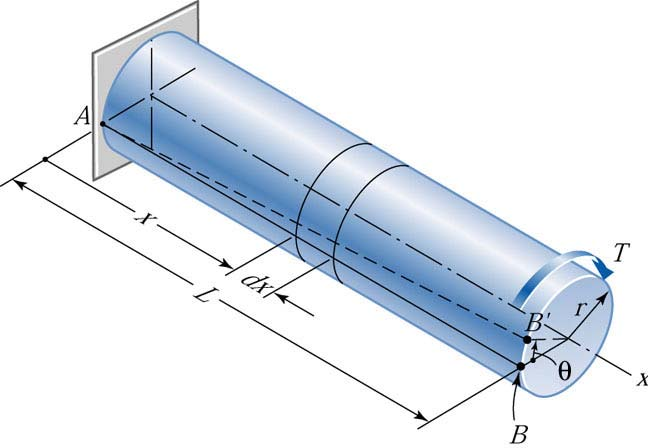
\includegraphics[width=\linewidth]{Ok.png}
		\caption{Circular beam subjected to torque T}
	\end{subfigure} \hspace{10mm}%to add space 
	\begin{subfigure}[b]{0.4\linewidth}
		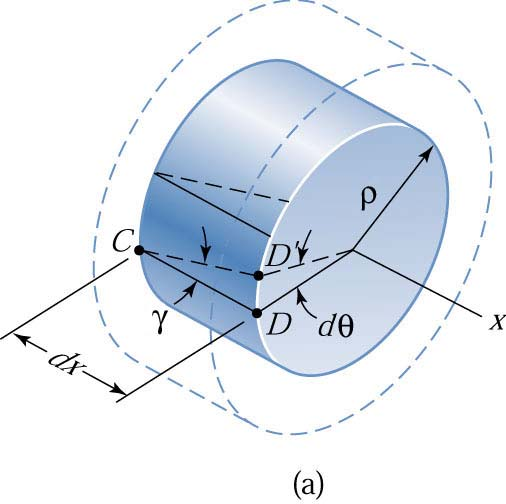
\includegraphics[width=\linewidth]{Ok1.png}
		\caption{dx section}
	\end{subfigure}
\end{figure}
\\
For a cylinder of diameter D and length l (see figure (a)), consider first a small annular element of mean radius rand thickness dx. The cylinder is subjected to a torque T, and this causes a circumferential shear stress T in the wall of the small element under consideration. If the torque is such that the left-hand end of this small element is twisted through an angle d$\theta$ in relation to the right-hand end, a longitudinal line AB on the surface of the element twists to position AB' (see figure (a)). For small angles of twist the shear strain $\gamma$ that is developed is given by
\begin{equation}
\gamma = \frac{BB'}{L}
\end{equation}
but arc BB' = r$\theta$ , therefore
\begin{equation}
\gamma = \frac{r\theta}{L}
\end{equation}
Within the elastic limit, the ratio of stress to strain is constant.
\thispagestyle{empty}	%To supress the printing of page number
\begin{equation}
\frac{\tau}{\gamma}=G
\end{equation}
G=\textit{Shear Modulus}\\
\\
\\
\\
Substituting for $\gamma$ from (2) in (3),and rearranging we have \\ \\
\begin{equation}
\frac{\tau}{r}=\frac{G\theta}{L}
\end{equation}
\\
For this small element, if the thickness dx is small, it can be assumed that the shear stress is constant across the thickness of the element. Also, if dx is small, the area of the section on which the shear stress $\tau$ acts approximates to 2$\pi$x dx. Hence, the total shear force acting on this element is $\tau$*(2$\pi$x dx).\\

The torque acting on this element is the moment of the tangential shear force about the longitudinal axis, and is T 2rrr2 dr. The torque T acting on the complete solid shaft is the sum of the moments of the tangential shear forces acting on all the small elements that go to make up the shaft, and is given by\\

\[ T= \int_{0}^{D/2}\tau2\pi x^2 dx\]

Substituting for $\tau$ from eqn(4), we have\\

\[T=\frac{G \theta}{L} \int_{0}^{D/2}2\pi x^3 dx\]

On solving we get\\
\[T=\frac{G \theta}{L}  \frac{\pi D^4}{32}\]

We know that for circular cross-section,\\
\[\frac{\pi D^4}{32}=J\]
\thispagestyle{empty}	%To supress the printing of page number
\\ \\

\thispagestyle{empty}	%To supress the printing of page number
\end{document}